% Figure: a story as a text vector (Attardo 2001, 2002).
% Generated by figures/text_figure.py; edit the script, not this file.
% Compile: pdflatex <this file>   Include: \includegraphics[width=\textwidth]{<pdf>}
\documentclass[border=4pt]{standalone}
\usepackage[T1]{fontenc}
\usepackage[scaled=0.92]{helvet}
\renewcommand{\familydefault}{\sfdefault}
\usepackage{xcolor}
\usepackage{tikz}
\usetikzlibrary{patterns}
\hyphenpenalty=10000 \exhyphenpenalty=10000
\begin{document}
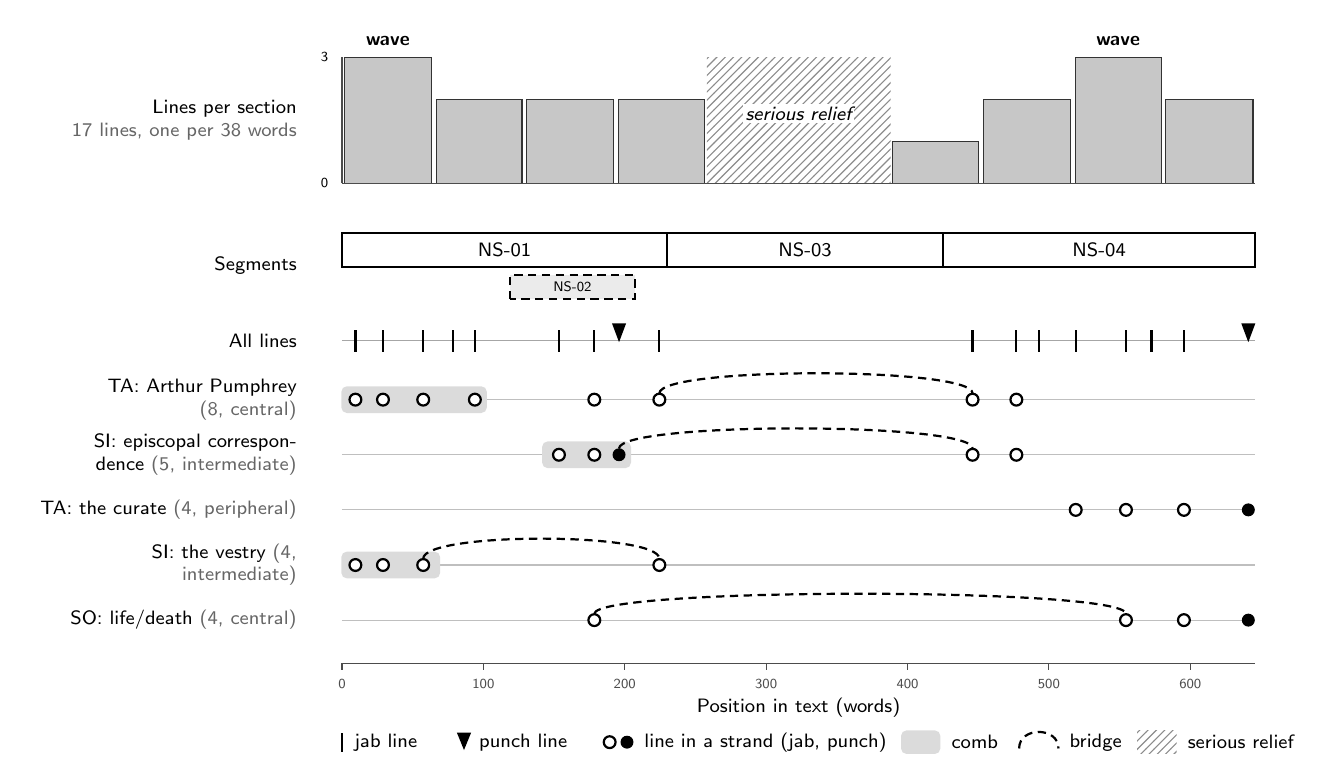
\begin{tikzpicture}[
  rowlabel/.style={font=\scriptsize, anchor=east, align=right, text width=3.3cm},
  legend/.style={font=\scriptsize, anchor=west, inner sep=1pt},
]
% Parameters: 10 sections; strands of >= 3 lines; central span >= 0.6, peripheral <= 0.3; comb gap <= 0.06; bridge gap >= 0.25 of the text.

% panel 1: humorous lines per section (10 sections)
\fill[pattern=north east lines, pattern color=black!45] (4.633,0.0) rectangle (6.967,1.600);
\filldraw[fill=black!22, draw=black!80, line width=0.4pt] (0.030,0.0) rectangle (1.137,1.600);
\filldraw[fill=black!22, draw=black!80, line width=0.4pt] (1.197,0.0) rectangle (2.286,1.067);
\filldraw[fill=black!22, draw=black!80, line width=0.4pt] (2.346,0.0) rectangle (3.454,1.067);
\filldraw[fill=black!22, draw=black!80, line width=0.4pt] (3.514,0.0) rectangle (4.603,1.067);
\filldraw[fill=black!22, draw=black!80, line width=0.4pt] (6.997,0.0) rectangle (8.086,0.533);
\filldraw[fill=black!22, draw=black!80, line width=0.4pt] (8.146,0.0) rectangle (9.254,1.067);
\filldraw[fill=black!22, draw=black!80, line width=0.4pt] (9.314,0.0) rectangle (10.403,1.600);
\filldraw[fill=black!22, draw=black!80, line width=0.4pt] (10.463,0.0) rectangle (11.570,1.067);
\node[font=\scriptsize\bfseries, anchor=south] at (0.584,1.620) {wave};
\node[font=\scriptsize\bfseries, anchor=south] at (9.858,1.620) {wave};
\node[font=\scriptsize\itshape, fill=white, inner sep=1pt] at (5.800,0.880) {serious relief};
\draw[black!70] (0.0,0.0) -- (11.6,0.0);
\draw[black!70] (0.0,0.0) -- (0.0,1.6);
\node[font=\tiny, anchor=east] at (-0.05,0.000) {0};
\node[font=\tiny, anchor=east] at (-0.05,1.600) {3};
\node[rowlabel] at (-0.45,0.8) {Lines per section\\\textcolor{black!60}{17 lines, one per 38 words}};
% panel 2: narrative segments
\draw[thick, fill=white] (0.000,-1.07) rectangle (4.130,-0.63);
\node[font=\scriptsize, text width=4.03cm, align=center] at (2.065,-0.85) {NS-01};
\draw[thick, fill=white] (4.130,-1.07) rectangle (7.632,-0.63);
\node[font=\scriptsize, text width=3.40cm, align=center] at (5.881,-0.85) {NS-03};
\draw[thick, fill=white] (7.632,-1.07) rectangle (11.600,-0.63);
\node[font=\scriptsize, text width=3.87cm, align=center] at (9.616,-0.85) {NS-04};
\draw[thick, densely dashed, fill=black!8] (2.137,-1.47) rectangle (3.717,-1.17);
\node[font=\tiny] at (2.927,-1.3199999999999998) {NS-02};
\node[rowlabel] at (-0.45,-1.05) {Segments};
% panel 3: every humorous line
\draw[black!35] (0.0,-2.0) -- (11.6,-2.0);
\draw[thick] (0.171,-2.14) -- (0.171,-1.8599999999999999);
\draw[thick] (0.521,-2.14) -- (0.521,-1.8599999999999999);
\draw[thick] (1.032,-2.14) -- (1.032,-1.8599999999999999);
\draw[thick] (1.409,-2.14) -- (1.409,-1.8599999999999999);
\draw[thick] (1.688,-2.14) -- (1.688,-1.8599999999999999);
\draw[thick] (2.756,-2.14) -- (2.756,-1.8599999999999999);
\draw[thick] (3.205,-2.14) -- (3.205,-1.8599999999999999);
\fill (3.519,-2.02) -- ++(-0.09,0.24) -- ++(0.18,0) -- cycle;
\draw[thick] (4.031,-2.14) -- (4.031,-1.8599999999999999);
\draw[thick] (8.009,-2.14) -- (8.009,-1.8599999999999999);
\draw[thick] (8.565,-2.14) -- (8.565,-1.8599999999999999);
\draw[thick] (8.853,-2.14) -- (8.853,-1.8599999999999999);
\draw[thick] (9.319,-2.14) -- (9.319,-1.8599999999999999);
\draw[thick] (9.957,-2.14) -- (9.957,-1.8599999999999999);
\draw[thick] (10.280,-2.14) -- (10.280,-1.8599999999999999);
\draw[thick] (10.693,-2.14) -- (10.693,-1.8599999999999999);
\fill (11.511,-2.02) -- ++(-0.09,0.24) -- ++(0.18,0) -- cycle;
\node[rowlabel] at (-0.45,-2.0) {All lines};
% panel 4: strands
\draw[black!25] (0.0,-2.75) -- (11.6,-2.75);
\fill[black!14, rounded corners=2pt] (-0.008,-2.92) rectangle (1.840,-2.58);
\draw[densely dashed, thick] (4.031,-2.67) .. controls (4.031,-2.33) and (8.009,-2.33) .. (8.009,-2.67);
\filldraw[fill=white, draw=black, thick] (0.171,-2.75) circle (0.075);
\filldraw[fill=white, draw=black, thick] (0.521,-2.75) circle (0.075);
\filldraw[fill=white, draw=black, thick] (1.032,-2.75) circle (0.075);
\filldraw[fill=white, draw=black, thick] (1.688,-2.75) circle (0.075);
\filldraw[fill=white, draw=black, thick] (3.205,-2.75) circle (0.075);
\filldraw[fill=white, draw=black, thick] (4.031,-2.75) circle (0.075);
\filldraw[fill=white, draw=black, thick] (8.009,-2.75) circle (0.075);
\filldraw[fill=white, draw=black, thick] (8.565,-2.75) circle (0.075);
\node[rowlabel] at (-0.45,-2.75) {TA: Arthur Pumphrey \textcolor{black!60}{(8, central)}};
\draw[black!25] (0.0,-3.45) -- (11.6,-3.45);
\fill[black!14, rounded corners=2pt] (2.542,-3.62) rectangle (3.671,-3.2800000000000002);
\draw[densely dashed, thick] (3.519,-3.37) .. controls (3.519,-3.0300000000000002) and (8.009,-3.0300000000000002) .. (8.009,-3.37);
\filldraw[fill=white, draw=black, thick] (2.756,-3.45) circle (0.075);
\filldraw[fill=white, draw=black, thick] (3.205,-3.45) circle (0.075);
\filldraw[fill=black] (3.519,-3.45) circle (0.075);
\filldraw[fill=white, draw=black, thick] (8.009,-3.45) circle (0.075);
\filldraw[fill=white, draw=black, thick] (8.565,-3.45) circle (0.075);
\node[rowlabel] at (-0.45,-3.45) {SI: episcopal correspondence \textcolor{black!60}{(5, intermediate)}};
\draw[black!25] (0.0,-4.15) -- (11.6,-4.15);
\filldraw[fill=white, draw=black, thick] (9.319,-4.15) circle (0.075);
\filldraw[fill=white, draw=black, thick] (9.957,-4.15) circle (0.075);
\filldraw[fill=white, draw=black, thick] (10.693,-4.15) circle (0.075);
\filldraw[fill=black] (11.511,-4.15) circle (0.075);
\node[rowlabel] at (-0.45,-4.15) {TA: the curate \textcolor{black!60}{(4, peripheral)}};
\draw[black!25] (0.0,-4.85) -- (11.6,-4.85);
\fill[black!14, rounded corners=2pt] (-0.008,-5.02) rectangle (1.247,-4.68);
\draw[densely dashed, thick] (1.032,-4.77) .. controls (1.032,-4.43) and (4.031,-4.43) .. (4.031,-4.77);
\filldraw[fill=white, draw=black, thick] (0.171,-4.85) circle (0.075);
\filldraw[fill=white, draw=black, thick] (0.521,-4.85) circle (0.075);
\filldraw[fill=white, draw=black, thick] (1.032,-4.85) circle (0.075);
\filldraw[fill=white, draw=black, thick] (4.031,-4.85) circle (0.075);
\node[rowlabel] at (-0.45,-4.85) {SI: the vestry \textcolor{black!60}{(4, intermediate)}};
\draw[black!25] (0.0,-5.55) -- (11.6,-5.55);
\draw[densely dashed, thick] (3.205,-5.47) .. controls (3.205,-5.13) and (9.957,-5.13) .. (9.957,-5.47);
\filldraw[fill=white, draw=black, thick] (3.205,-5.55) circle (0.075);
\filldraw[fill=white, draw=black, thick] (9.957,-5.55) circle (0.075);
\filldraw[fill=white, draw=black, thick] (10.693,-5.55) circle (0.075);
\filldraw[fill=black] (11.511,-5.55) circle (0.075);
\node[rowlabel] at (-0.45,-5.55) {SO: life/death \textcolor{black!60}{(4, central)}};
\draw[black!70] (0.0,-6.1) -- (11.6,-6.1);
\draw[black!70] (0.000,-6.1) -- ++(0,-0.08) node[below, font=\tiny] {0};
\draw[black!70] (1.796,-6.1) -- ++(0,-0.08) node[below, font=\tiny] {100};
\draw[black!70] (3.591,-6.1) -- ++(0,-0.08) node[below, font=\tiny] {200};
\draw[black!70] (5.387,-6.1) -- ++(0,-0.08) node[below, font=\tiny] {300};
\draw[black!70] (7.183,-6.1) -- ++(0,-0.08) node[below, font=\tiny] {400};
\draw[black!70] (8.978,-6.1) -- ++(0,-0.08) node[below, font=\tiny] {500};
\draw[black!70] (10.774,-6.1) -- ++(0,-0.08) node[below, font=\tiny] {600};
\node[font=\scriptsize, anchor=north] at (5.8,-6.42) {Position in text (words)};
% legend
\draw[thick] (0.0,-7.22) -- (0.0,-6.9799999999999995); \node[legend] at (0.12,-7.1) {jab line};
\fill (1.55,-7.199999999999999) -- ++(-0.09,0.22) -- ++(0.18,0) -- cycle; \node[legend] at (1.7,-7.1) {punch line};
\filldraw[fill=white, draw=black, thick] (3.4,-7.1) circle (0.075); \filldraw[fill=black] (3.62,-7.1) circle (0.075); \node[legend] at (3.8,-7.1) {line in a strand (jab, punch)};
\fill[black!14, rounded corners=2pt] (7.1,-7.25) rectangle (7.6,-6.949999999999999); \node[legend] at (7.7,-7.1) {comb};
\draw[densely dashed, thick] (8.6,-7.18) .. controls (8.6,-6.8999999999999995) and (9.1,-6.8999999999999995) .. (9.1,-7.18); \node[legend] at (9.2,-7.1) {bridge};
\fill[pattern=north east lines, pattern color=black!45] (10.1,-7.25) rectangle (10.6,-6.949999999999999); \node[legend] at (10.7,-7.1) {serious relief};
\end{tikzpicture}
\end{document}
